%\documentclass[12pt]{article}
\documentclass[12pt]{revtex4}
%\documentclass[draft,12pt]{article}
\usepackage{amsmath}
\usepackage{amsfonts}
\usepackage{amsbsy}
\usepackage{lscape} 
\usepackage{color}
\usepackage{graphicx,epsfig}
\usepackage[english]{babel}
\usepackage{latexsym}
\usepackage{amssymb}
\usepackage{palatino}
%\usepackage{chancery}
%\usepackage{newcent}
%\usepackage{charter}
%\usepackage{zapfchan}
%\usepackage{bookman}
%\usepackage{sparticles}        %Package for displaying sparticle names. 
%\usepackage{feynmf}            %Package for feynman diagrams. 

\newcommand{\beq}{\begin{equation}}
\newcommand{\eeq}{\end{equation}}

\newcommand{\eq}{{\rm eq}}
\newcommand{\lgr}{\left\lgroup}
\newcommand{\rgr}{\right\rgroup}
\newcommand{\Mpl}{M_{\rm Pl}}
\newcommand{\Tfr}{T_{\rm fr}}
\newcommand{\Tsph}{T_{\rm sph}}
\newcommand{\Gsph}{\Gamma_{\rm sph}}
\newcommand{\Lray}{\Lambda_{\rm ray}}

\newcommand{\p}{\partial}
\newcommand{\mc}[1]{\mathcal{#1}}
\newcommand{\md}{\mathcal{D}}
\newcommand{\wt}{\widetilde}
\newcommand{\ov}{\overline}
\newcommand{\suc}{{\rm SU}_{\rm C}(3)}
\newcommand{\sul}{{\rm SU}_{\rm L}(2)}
\newcommand{\ue}{{\rm U}(1)}
\newcommand{\GeV}{{\rm GeV}}
\newcommand{\eV}{{\rm eV}}
%\newcommand{\su3}{{\rm SU}_{\rm C}(3)}

%%%%%%%%%%%%%%%%%%%%%%%%%%%%%%%%%%%%%%%
%  Slash character...
\def\slashed#1{\setbox0=\hbox{$#1$}             % set a box for #1
   \dimen0=\wd0                                 % and get its size
   \setbox1=\hbox{/} \dimen1=\wd1               % get size of /
   \ifdim\dimen0>\dimen1                        % #1 is bigger
      \rlap{\hbox to \dimen0{\hfil/\hfil}}      % so center / in box
      #1                                        % and print #1
   \else                                        % / is bigger
      \rlap{\hbox to \dimen1{\hfil$#1$\hfil}}   % so center #1
      /                                         % and print /
   \fi}                                        %

%%EXAMPLE:  $\slashed{E}$ or $\slashed{E}_{t}$


\begin{document}

%%
%% The title page
%% 
\begin{titlepage}
\renewcommand{\thefootnote}{\fnsymbol{footnote}}

\vspace*{3.0cm}
\begin{center}
{\Large
  \textbf{
  \textsc{CPT-odd Leptogenesis}
         }
      }

\vspace*{1.0cm}
  {\large \fontfamily{ppl}\selectfont Pavel A. Bolokhov~ 
        {\normalsize\bf \textsc{and}} ~Maxim Pospelov}

\vspace*{1.5cm}
{\large\bf Abstract}
%       We introduce Lorentz violating interactions at dimension five level into
%       the Standard Model.
\end{center}

        We show that modification of theory with CPT-odd interactions..

\end{titlepage}

%%%%%%%%%%%%%%%%%%%%%%%%%%%%%%%%%%%%%%%%%%%%%%%%%%%%%%%%%%%%%%%%%%%%%%
%%%%%%%%%%%%%%%%%%%%%%%%%%%%%%%%%%%%%%%%%%%%%%%%%%%%%%%%%%%%%%%%%%%%%%
%
%                            INTRODUCTION
%
%%%%%%%%%%%%%%%%%%%%%%%%%%%%%%%%%%%%%%%%%%%%%%%%%%%%%%%%%%%%%%%%%%%%%%
%%%%%%%%%%%%%%%%%%%%%%%%%%%%%%%%%%%%%%%%%%%%%%%%%%%%%%%%%%%%%%%%%%%%%%
\section{Introduction}

%---	Sakharov's conditions
%
%---	reference to Kostelecky's paper
%
%---	Features of CPT-odd leptogenesis, including equilibrium distribution
%
%---	Leptogenesis epoch, sphaleron epoch
%
%---	unnecessity to having more than one heavy neutrinos
%
%---	Declare analysis of Boltzmann equations for operators of 
%	dimension five, and general arguments for higher-dimensional
%	operator
%
%---	Heavy neutrino interaction, effective lagrangian


	It is known that CPT-odd perturbations of a theory can effectively
	replace two Sakharov's conditions for baryogenesis: violation of CP
	invariance and the absence of thermal equilibrium.
	The main reason for this is that baryon asymmetry is present in the
	equilibrium plasma due to the CPT-odd shifts of the dispersion relations
	for baryons.
	That means that, as long as one has a CPT-odd model with baryons in equilibrium,
	the BAU is guarranteed to be generated.
	In some sense the problem of BAU becomes somewhat trivial: one only has
	to add proper perturbations to the theory.
	
	One, however, still has the problem of B-nonconservation: to keep the plasma
	in equilibrium one needs B-violating processes, which do not exist in the
	Standard Model.
	There are well-known solutions to this problem which extend slightly beyond
	the Standard Model, for example, into GUTs, where the baryon number is not
	conserved.
%such that B-violating processes 
%	can proceed.
	It is easy then to compute the equilibrium number density of baryons.

	CPT-odd baryogenesis has already been covered in the literature [Carrol,Kostelecky].
	One of the important goals is to connect the observed BAU with the existing constraints
	on LV interactions, which was ?partly? done in [Kostelecky]. 
	However, to present a more detailed numerical prediction for baryon asymmetry, 
	one needs to take into consideration the kinetic equations for baryon number density,
	as baryon-violating processes not always were in equilibrium.
	We concentrate on CPT-odd interactions of mass dimension five.
	Lower dimensional operators are in potential conflict with phenomenology, whereas
	dimension five LV is claimed to be capable of producing the BAU.
	
	The main direction of the present work is to consider generation of BAU via CPT-odd
	leptogenesis.
%	One of the attracting models of baryogenesis is leptogenesis.
	In contrast with baryogenesis models, which as a rule require higher gauge groups 
	and therefore involve much more new degrees of freedom, leptogenesis only
	requires heavy majorana neutrinos, which simultaneously provide small
	masses for observed neutrinos.
	We introduce CPT-odd interactions into the lepton sector of the Standard Model:
\begin{equation}
\label{LV}
	\mathcal{L}_{LV} ~~=~~ \eta^{\mu\nu\rho}\cdot \ov{L}\gamma_\mu \md_\nu \md_\rho L~.
\end{equation}
	The zeroth component of the tensor $ \eta^{\mu\nu\rho} $, $ \eta^{000} \equiv \eta $ provides a 
	shift for the dispersion relations for leptons and antileptons, with different signs. 
	Therefore, a surplus of particles over antiparticles is created when leptons are
	in thermal equilibrium.
	It is noteable, that such perturbations allow for successful leptogenesis already
	with one flavor of majorana neutrinos, whereas conventional leptogenesis requires
	at least two of them [ref].
	
	The major part of leptogenesis occurs when majorana neutrinos have decayed,
	and only existed off-shell, mediating lepton number violating processes.
	These processes maintain the equilibrium value for 
	lepton number asymmetry. 
	The Lagrangian for heavy neutrinos looks as
\begin{equation}
	\mathcal{L}  ~~\supset~~ -\,\frac 12\, M_R\, \ov{N}N ~~+~~
				Y\cdot \ov{L}HN ~~+~~  Y^\dagger\cdot \ov{N}H^\dagger L~,
\end{equation}
	where $ Y $ are Yukawa couplings.
	We switch to Weyl spinors for convenience, in which the Lagrangian can be rewritten as
\begin{equation}
	\mathcal{L}  ~~\supset~~ 
	-\,\frac 12\, M_R\, \left( \lambda\lambda ~+~ \ov{\lambda\lambda} \right) ~~+~~
				Y\cdot \ov{L\lambda}H ~~+~~  Y^\dagger\cdot H^\dagger \lambda L~,
\end{equation}
	where
\[	
	N  ~~=~~ \left\lgroup 
		\begin{matrix}
			\lambda_\alpha \\
			\ov{\lambda}^{\dot{\alpha}}
		\end{matrix}
		\right\rgroup~.
\]
	Integrating out the majorana neutrinos, one obtains an effective L-violating vertex:
\begin{equation}
\label{L_eff}
	\mathcal{L}_{\rm eff} ~~=~~ \frac{Y^\dag Y^\dag}{2\, M_R} \, H^\dag L^\alpha H^\dag L_\alpha~.
\end{equation}
	This interaction induces L-violating processes which determine the lepton asymmetry
	until the lepton freeze-out.
	Sphaleron processes then convert the lepton abundance into the baryon asymmetry which
	should have persisted up to now.

	We examine closely the kinetic equations for the L-violating processes and argue that
	the freeze-out temperature lies very close to the sphaleron ignition temperature, such
	that analysis of their simultaneous contributions is needed. 
	We adjust the coupling constant $ \eta $ in \eqref{LV} in such a way as to produce 
	the observed value of the baryon asymmetry and compare the results with the existing
	limits on LV interactions. 
	We argue that, the bounds on LV from observations of high energy cosmic rays renders
	CPT-odd leptogenesis impossible for models with operators of mass dimension five \eqref{LV}, 
	as well as for models with higher-dimensional operators.
	
	{\it How did Kostelecky then obtained the observed BAU?}
	

%%%%%%%%%%%%%%%%%%%%%%%%%%%%%%%%%%%%%%%%%%%%%%%%%%%%%%%%%%%%%%%%%%%%%%
%%%%%%%%%%%%%%%%%%%%%%%%%%%%%%%%%%%%%%%%%%%%%%%%%%%%%%%%%%%%%%%%%%%%%%
%
%              REACTION RATES AND BOLTZMANN EQUATIONS     
%
%%%%%%%%%%%%%%%%%%%%%%%%%%%%%%%%%%%%%%%%%%%%%%%%%%%%%%%%%%%%%%%%%%%%%%
%%%%%%%%%%%%%%%%%%%%%%%%%%%%%%%%%%%%%%%%%%%%%%%%%%%%%%%%%%%%%%%%%%%%%%
\section{Reaction rates and Boltzmann equations}

\subsection{Simple kinetic equation}

Introduction of the CPT-odd interactions leads to the modification of 
dispersion relations for leptons
\[
	E_L(p) ~~=~~ |\vec{p}| ~+~ \frac 12\, \eta_L\, \vec{p}^2~,
\]
which we may assume massless at the temperatures of leptogenesis.
This, in its turn leads to a shift of the equilibrium number density
from zero to some small number
\[
        n_L^\eq ~~=~~ \frac{g_L}{\pi^2 \beta^3}
			\left (\, 1 ~-~ \frac{6\,\eta_L}{\beta} \,\right)~.
\]
By itself, this modification would not cause a non-zero lepton density
of plasma. 
However, much in accord with the standard leptogenesis scenario, the 
effective interaction vertices of lepton and higgs fields,
obtained by integrating out heavy majorana neutrinos, made possible
for exchange processes to exist at temperatures slightly below the
majorana neutrino scale $ M $.
These processes (L-processes from now on) flipped leptons into antileptons, 
and, provided their
rate was higher than the Hubble expansion rate, maintained the equilibrium
of lepton number density.
At lower temperatures, the Hubble rate started to dominate, and the
lepton-flipping processes were not fast enough to track the decrease
of 
%the equilibrium number density with 
the temperature. 
As in standard baryogenesis, the frozen number density can be roughly
estimated by evaluating the equilibrium density at the temperature
of the freeze-out.


\begin{figure}
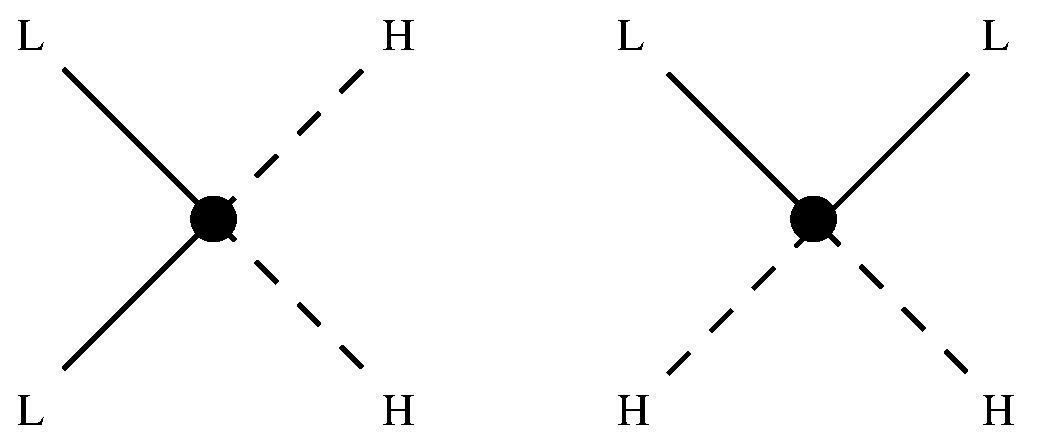
\includegraphics[width=9cm]{lflip.eps}
\caption{L-flipping processes generated by the effective vertex \eqref{L_eff}.}
\label{lflip_fig}
\end{figure}
There are two types of interactions generated by the effective
Lepton-Higgs vertex, see Fig.~\ref{lflip_fig}.
They generate the following processes relevant for leptogenesis:
\begin{align}
\notag
	L~~+~~L ~~\rightarrow~~ H~~+~~H~  \\
\notag
	L~~+~~\ov{H} ~~\rightarrow~~ \ov{L}~~+~~H~,
\end{align}
together with their inverse processes, and with the same set of processes
for antileptons.
However, since our CPT-odd interactions are T-invariant, the amplitudes for
direct and inverse processes are equal, and we therefore have 
only three different amplitudes, which we call  
$ A_{LL} $, $ A_{\ov{LL}} $ and $ A_{LH} $.
Denoting the corresponding reaction volumes by
$ W_{LL} $, $ W_{\ov{LL}} $, $ W_{L\ov{H}} $ and $ \ov{W}_{L\ov{H}} $,
where 
\begin{align*}
% first line
	W_{LL}   ~~=~~  &
		\int d\pi_p d\pi_q d\pi_k d\pi_r ~
		(2\pi)^4~ \delta^4 ( p + q - k - r )\,
		| A_{LL} |^2\, f_L^\eq(p)\, f_L^\eq(q)~, \\
% second line
	W_{\ov{LL}}   ~~=~~  &
		\int d\pi_p d\pi_q d\pi_k d\pi_r ~
		(2\pi)^4~ \delta^4 ( p + q - k - r )\,
		| A_{L\ov{H}} |^2\, f_L^\eq(p)\, f_{\ov{H}}^\eq(q)~, \\
% third line
	W_{L\ov{H}}  ~~=~~  &
		\int d\pi_p d\pi_q d\pi_k d\pi_r ~
		(2\pi)^4~ \delta^4 ( p + q - k - r )\,
		| A_{L\ov{H}} |^2\, f_{\ov{L}}^\eq(p)\, f_H^\eq(q)~, \\
% fourth line
	\ov{W}_{L\ov{H}}  ~~=~~  &
		\int d\pi_p d\pi_q d\pi_k d\pi_r ~
		(2\pi)^4~ \delta^4 ( p + q - k - r )\,
		| A_{LL} |^2\, f_{\ov{L}}^\eq(p)\, f_{\ov{L}}^\eq(q)~,
\end{align*}
	we can write the Boltzmann equations for the lepton number density
	as
\begin{equation*}
\left\{~~
\begin{split}
% first line
	\lgr \p_t ~+~ 3H \rgr 
		n_L ~~=~~ &
	-\, 2\, W_{LL} \lgr \frac{n_L^2}{(n_L^\eq)^2} ~-~ 1 \rgr
	~~-~~
	W_{L\ov{H}} \lgr \frac{n_L}{n_L^\eq} ~-~ 
			\frac{n_{\ov{L}}}{n_{\ov{L}}^\eq} \rgr  \\
% second line
	\lgr \p_t ~+~ 3H \rgr 
		n_{\ov{L}} ~~=~~ &
	-\, 2\, W_{\ov{LL}} \lgr 
		\frac{n_{\ov{L}}^2}{(n_{\ov{L}}^\eq)^2} ~-~ 1 \rgr
	~~-~~
	\ov{W}_{L\ov{H}} \lgr \frac{n_{\ov{L}}}{n_{\ov{L}}^\eq} ~-~ 
			\frac{n_L}{n_L^\eq} \rgr  \\
\end{split}
\right._{~.}
\end{equation*}
	The factor of two in the RHS here reflects that the LL processes
	change the number of leptons by two ({\it Hmm... what about LH processes?}).
	The first thing to note is that even though we could have introduced
	a modification for the dispersion relations for the higgs, 
	its parameter would not enter the equations for the lepton number
	density (just because the higgs equilibrium number density completely
	dropped out of the right hand side of ...).
	
	Next we make the customary and a well-justified assumption of 
	smallness of the chemical potential for leptons,
\[
	\frac{n_L}{n_L^\eq} ~~=~~ e^{\mu/T} ~~\simeq~~ 1 ~~+~~ \mu/T~,
\]
	which enables us now to linearize the equations in $ \mu $.

	The kinetic equations for $ n_L $ now look as
\begin{equation}
\label{kinetic_eqn_prelim}
\begin{split}
% first line
	\Bigl\{ \p_t ~+~ 3H \Bigr\}
		n_L ~~=~~ & 
	-\, \lgr 4\, W_{LL} ~+~ 2\, W_{L\ov{H}} \rgr  \mu/T \\
% second line
	\Bigl\{ \p_t ~+~ 3H \Bigr\} 
		n_{\ov{L}} ~~=~~ &
	\phantom{-\,}
	\lgr 4\, W_{\ov{LL}} ~+~ 2\, \ov{W}_{L\ov{H}} \rgr  \mu/T ~.
\end{split}
\end{equation}

	Now we observe, that due to smallness of the chemical potential
	any CPT-odd effects in the reaction rates can be neglected.
	There are two imaginable sources of CPT-odd contributions 
	to the reaction rates: modified dispersion relations and 
	CPT-odd modifications of Lepton-Higgs vertices. 
	In our case, neither of them contribute, so we can take
	$ W_{\ov{LL}} = W_{LL} $ and
	$ \ov{W}_{L\ov{H}} = W_{L\ov{H}} $.

	From the above equations we only need their difference, the actual
	lepton asymmetry.
	For convenience, we express the equilibrium number density in terms
	of the unmodified number density 
	$ n_L^0 = g_L/\pi^2 \cdot T^3 $
\[
	n_{L,\ov{L}}^\eq ~~=~~ n_L^0\, \left(\, 1 ~\pm~ \theta_L T \,\right)~,
\]
	where $ \theta_L = -6\, \eta_L $.
	The lepton asymmetry $ Y_L $ then can be expressed as
\[
	n_L ~~-~~ n_{\ov{L}} ~~\equiv~~ 2\, n_L^0 \cdot Y_L~,
	\qquad\quad Y_L ~~=~~ \mu/T ~~+~~ \theta_L T~.
\]
	
	We also introduce dimensionless parameters $ \alpha $, 
	$ \delta $ and $ \gamma $, by separating out the massive
	parameters from the quantities entering the kinetic equation:
\begin{align*}
% first line
&	 n_L^0 ~~=~~   \delta \cdot T^3~, \\
% second line
&	H     ~~=~~   \frac{T^2}{2\, \alpha\, \Mpl}~, \\
% third line
&	4\, W_{LL} ~~+~~ W_{L\ov{H}} ~~=~~ 
		 \gamma\, \frac{T^6}{M_R^2}~, \\
% fourth line
&	\lambda ~~\equiv~~  \frac{2\,\alpha\,\gamma}{\delta} ~.
\end{align*}
	The explicit values of the above constants are
	$ \alpha  ~=~ 0.3\, g_*^{-1/2} $ and 
	$ \delta  ~=~ g_L/\pi^2 $.
%\begin{align*}
%% first line
%	\alpha & ~~=~~ 0.3\, g_*^{-1/2}~, \\
%% third line
%	\delta & ~~=~~ \frac{g_L}{\pi^2}~.
%\end{align*}
	The value of $ \gamma $ is determined by the explicit 
	cross-sections of the lepton-number flipping processes
	(see Fig.~\ref{lflip_fig}):
\[
	\gamma  ~~=~~ \frac{3}{2\pi^2}\, (N_g)^2\, |Y|^4~, \\
\]
	where $ N_g = 3 $ is the number of generations of leptons.
	Then the kinetic equation takes the simple form
\begin{equation}
\label{btz_simple}
	Y_L' ~~=~~ \frac{\lambda\,\Mpl}{M_R^2} \,
			\lgr Y_L ~-~ \theta_L\, T \rgr~,
\end{equation}
	where the prime indicates differentiation with respect to
	the temperature.
	
	The general solution of \eqref{btz_simple} is
\[
	Y_L^{(\rm g)} ~~=~~ \frac{\theta_L\,M_R^2}{\lambda\,\Mpl}
		~+~ \theta_L\,T ~+~
		A\cdot e^{\frac{\lambda\, \Mpl}{M_R^2}\, T}~,
\]
	with an arbitrary constant $ A $.
	Requiring $ Y_L $ to stay close to its equilibrium value 
	$ \theta_L\, T $ at high temperatures one has to 
% presume that 
	put $ A = 0 $:
\begin{equation}
\label{btz_sol_simple}
	Y_L ~~=~~ \frac{\theta_L\,M_R^2}{\lambda\,\Mpl}
		~+~ \theta_L\,T ~
\end{equation}
	(one might worry why we have been able to obtain a special
	solution of equation \eqref{btz_simple} without essentially giving it
	any input data; note, however, that in the sense of leptogenesis
	the solution \eqref{btz_sol_simple} still has an arbitrary
	constant $ M_R $ which has to be fixed).
	Now, Eq.~\eqref{btz_sol_simple} provides us with the freeze-out
	temperature
\begin{equation}
\label{T_R}
	\Tfr ~~\sim~~ \frac{M_R^2}{\lambda\,\Mpl}~,
\end{equation}
	as well as with an estimate for the frozen number density
\begin{equation}
\label{Y_L_simple}
	Y_L^{\rm fr} ~~\sim~~ \frac{\theta_L\,M_R^2}{\lambda\,\Mpl}~.
\end{equation}
	This is of course the temperature at which the Hubble rate equals 
	the L-process rate.
	We emphasize that \eqref{Y_L_simple} is only an estimate, 
	and one needs a more careful numerical analysis for the final
	result.
	In any case, it is not $ Y_L $ that is of interest, but, rather,
	the corresponding baryon asymmetry $ Y_B $.
	In accord with the standard leptogenesis, sphalerons diffuse
	half of the lepton number yield into the baryon number.


	One then is faced with three possible developments of the scenario.
	The first one appears if $ \Tsph $, the temperature at which
	sphaleron processes become rapid, is considerably lower than $ T_R $.
%	As is well-known, the sphalerons turn half of the lepton number
%	into baryon number.
	In this case, during the leptogenesis epoch, 
	i.e. at $ M_R > T > T_R $,
	the sphalerons were very slow and could essentially be dropped 
	from consideration,
	thus leaving one with \eqref{Y_L_simple} as the lepton number yield.
	Below $ T_R $, the lepton number stayed constant, as the 
	lepton-flipping processes were too slow to keep equilibrium.
	And, finally, at $ \Tsph $, the sphalerons kicked in and diffused
	half of the lepton number \eqref{Y_L_simple} into the baryon number.

	The second possibility arises if the sphaleron age partially
	overlaps the leptogenesis epoch, i.e. if $ \Tsph \gtrsim T_R $.
	If $ \Tsph $ happens to be enough greater than $ T_R $, there
	existed a period during which both processes were in equilibrium.
	[{\it
	Qualitatively, one can estimate the resulting BAU as follows.
	Fast lepton-switching processes kept the lepton number around
	its equilibrium, while sphalerons brought the baryon number to
	the same level.
	Indeed, sphalerons do not change $ B - L $. 
	Since heavy-neutrino-mediated processes changed $ L $ 
	(and did not touch $ B $), the sphalerons had to adjust $ B $ 
	accordingly. 
	At temperature $ T_R $, the ``leptogenesis'' stopped, 
	the lepton number froze at the level estimated by \eqref{Y_L_simple},
	and the BAU must have been of the same level. 
	}]
	To estimate the resulting BAU it is easier to switch to the
	basis of $ B + L $ - and $ B - L $ -violating operators.
	In this language, L-processes generate both  $ B + L $ and $ B - L $:
\[
	Y_{B-L} ~\simeq~ \frac 12 (\theta_B - \theta_L ) \cdot T_R~,\qquad
	Y_{B+L} ~\simeq~ \frac 12 (\theta_B + \theta_L ) \cdot T_R~.
\]	
	Sphalerons then wash out $ Y_{B+L} $, yielding the BAU to be
	$ \frac 12 (\theta_B - \theta_L ) \cdot T_R $.
	Note that $ \theta_L $ gives the same contribution here as in the 
	first case.
	Opposite to $ \theta_B $, which did not contribute in the first case
	due to the absence of B-flipping processes.
	
	The third case corresponds to $ \Tsph \approx T_R $.
	Then there was no epoch during which both processes
	were in equilibrium, and in this sense this case is more complicated.
	However, to get an estimate, the straighforward reasoning is
	still the same.
	Whatever $ B $ and $ L $ at $ T = \Tsph $ were, the resulting
	lepton and baryon asymmetry after the sphaleron epoch only
	depended on the input $ B - L $.
	Of course, since L-processes only changed the lepton number,
	this $ B - L $ at  $ T \sim \Tsph \approx T_R $ can 
	again be estimated by \eqref{Y_L_simple}.
	It is clear, however, that this estimate is rather crude and 
	one needs a more direct numerical analysis to obtain an actual
	number.
	

\subsection{Account for the sphaleron rate}

	We now turn to Eq.\eqref{T_R}, which determines the time when
	the lepton-flipping processes became slower than the Hubble
	rate.
	To get an upper limit on $ T_R $, one can use the atmospheric
	limit on neutrino masses, $ m_\nu^i > 0.05~\eV $ 
	to estimate the ratio $ M_R^2 / Y^4 $.
	For $ M_R \sim 10^{15}~\GeV $ one obtains temperature $ T_R^{max} $ 
	of the order $ 10^{13}~\GeV $.
	To get a lower limit on $ T_R $, one can use the cosmological
	bound on total neutrino masses
\[
	\sum (m_i)^2 ~~\leq~~ (0.65~\eV)^2~,
\]
	which yields $ T_R^{min} $ of the order of $ 10^{11}~\GeV $. 
	It is estimated that $ \Tsph \sim 10^{12}~\GeV $ [ref]. 
	One can see that typical values of parameters at best 
	lead to $ T_R $ being slightly greater than $ \Tsph $.
	It is most likely then, that there was no period when
	both sphalerons and L-processes were active, but at the same
	time, there was no separation between the characteristic 
	temperatures of their activity.
	That means that neither of the processes can be neglected,
	what corresponds to the third scenario introduced above.
%	One can see that reasonable parameters yield the third scenario
%	described above.
	To obtain a quantified prediction for BAU one certainly needs
	to consider carefully both sphaleron processes and L-processes
	in the kinetic equations.

	For our purposes it will be sufficient to use the linear
	temperature dependence approximation of the sphaleron rate [ref]. 
	The general effect of sphalerons is to partly wash-out $ B + L $,
	while keeping $ B - L $ intact.
	Schematically, the sphaleron contribution to the Boltzmann equation
	for $ n_L $, $ n_B $ is [KRS,Moore]:
\begin{equation}
\label{sph_corr}
	\frac{d}{dt}\, n_B~,~~
	\frac{d}{dt}\, n_L
	~~~\supset~~~ -\, \Gsph 
		\lgr   n_B - n_B^\eq \;~+~\;
		       n_L - n_L^\eq 
		\rgr~,
\end{equation}
	where
\[
	\Gsph ~~\simeq~~ \frac{39}{4}\,\omega T~, \qquad\qquad 
	{\rm ~with~}
	\omega ~~\simeq~~ \,10^{-6}~.
\]
	One then includes the account for the sphaleron rate \eqref{sph_corr}
	into the kinetic equations \eqref{kinetic_eqn_prelim}.
	Also, one has to add similar equations for the baryon density $ n_B $.
	Instead of working with the measures of asymmetry $ Y_L $ and 
	 $ Y_B $ it is technically more convenient to introduce the
	deviation from equilibrium $ \Upsilon_{L,B} $:
\[
	\Upsilon_i ~~=~~ Y_i ~-~ \theta_i T ~~=~~ \mu_i/T~,
	\qquad\qquad i~=~L,B~.
\]
	(now that we are tracking both lepton and baryon numbers 
	simultaneously, we have to explicitly indicate which quantites
	are related to which sector, and therefore we will be appending
	a subscript L or B where appropriate).
	In terms of $ \Upsilon_{L,B} $
	the kinetic equations can be written in a more symmetric way:
\begin{equation}
\label{eqn_ups}
\left\{~~
\begin{split}
% first line
	\delta_L \lgr \Upsilon_L' ~~+~~ \theta_L \rgr
	& ~~\;=~~\;
	2\, \alpha\chi \Mpl \cdot T^{-2} 
	\lgr \delta_L \Upsilon_L ~~+~~ \delta_B \Upsilon_B \rgr 
	\;~~+~~\;
	2\, \alpha\gamma\, \frac{\Mpl}{M_R^2} \cdot \Upsilon_L \\
% second line
	\delta_B \lgr \Upsilon_B' ~~+~~ \theta_B \rgr
	& ~~\;=~~\;
	2\, \alpha\chi \Mpl \cdot T^{-2} 
	\lgr \delta_L \Upsilon_L ~~+~~ \delta_B \Upsilon_B \rgr 
	~~.
\end{split}
\right.
\end{equation}
	This is a purely technical simplification, since
	the quantity of interest is the baryon asymmetry normalized on the
	entropy density at the present time, which is still expressed
	in terms of $ Y_B $,
\begin{equation}
\label{def_asy}
	\mathfrak{a}_B ~~=~~ 7.04\, \frac{45}{\pi^4}\, \frac{g_B}{g_*}\, Y_B
		~~\equiv~~ (\, 6.1 ~\pm~ 0.3 \,)\times 10^{-10}~.
\end{equation}

	One now has to solve system \eqref{eqn_ups} numerically.
	It is reasonable to impose initial condition at the temperatures
	where the essential part of leptogenesis begins, which we
	take to be $ M_R = 10^{15}~\GeV $.
	At these temperatures, leptons were in their equilibrium, which
	had a nonzero value of the lepton number defined by $ \eta_L $.
	As we have seen, this hypothesis is quite sensible since 
	the freeze-out temperature $ T_R $ is sufficiently smaller than
	$ M_R $.
	Even if we start off out of equilibrium, the fast L-processes
	will quickly bring the system back into it.
	Consequently, if we take the initial leptogenesis temperature
	to be some $ T ~=~ M ~>~ M_R $, then at $ T~=~M_R $ one would
	still have equilibrium in the lepton sector, so the above
	choice of the leptogenesis temperature is quite justified.

	As for baryons, we are less legitimate to assume them to be in
	equilibrium, since at those times there were no baryon number
	violating processes to maintain it.
	Theoretically their initial asymmetry could have been arbitrary,
	but aesthetically it is more natural to assume it zero
	(otherwise the whole problem of obtaining a non-zero BAU would
	not be much contented):
\begin{align*}
	Y_L\bigl|_{M_R} & ~~=~~ \theta_L\, M_R~, \\
	Y_B\bigl|_{M_R} & ~~=~~ 0~.
\end{align*}
		


%%%%%%%%%%%%%%%%%%%%%%%%%%%%%%%%%%%%%%%%%%%%%%%%%%%%%%%%%%%%%%%%%%%%%%
%%%%%%%%%%%%%%%%%%%%%%%%%%%%%%%%%%%%%%%%%%%%%%%%%%%%%%%%%%%%%%%%%%%%%%
%
%        BARYON ASYMMETRY OF THE UNIVERSE: SUPPLY AND DEMAND  
%
%%%%%%%%%%%%%%%%%%%%%%%%%%%%%%%%%%%%%%%%%%%%%%%%%%%%%%%%%%%%%%%%%%%%%%
%%%%%%%%%%%%%%%%%%%%%%%%%%%%%%%%%%%%%%%%%%%%%%%%%%%%%%%%%%%%%%%%%%%%%%
\section{Baryon Asymmetry of the Universe: ~Supply and Demand}

	We set up the problem inverse to the Cauchy problem:
%	given the present-time baryon abundance \eqref{def_asy},
	we set to find the values of $ \eta_L $ and $ \eta_B $ 
	big enough to generate the present-time baryon 
	abundance \eqref{def_asy}.
	Since equations \eqref{eqn_ups} are linear in $ \Upsilon_i $,
	it will be sufficient to consider two opposite cases
\[
	\eta_L ~~\neq~~ 0,\qquad\qquad \eta_B ~~=~~ 0~, 
\]
	and
\[
	\eta_L ~~=~~ 0,\qquad\qquad \eta_B ~~\neq~~ 0~.
\]
	Qualitative features of the solution of Eq.~\eqref{eqn_ups} can
	be inferred only in an assumption of small sphaleron rate,
	which unfortunately is only approximately true.
	The first case should be close to the scenario considered in
	section X.X --- 
	leptons freeze out, and at lower temperatures get converted
	into baryons. 
	The resulting BAU thus should weakly depend on the sphaleron
	rate.

	For the second case, the sphaleron rate is more crucial, since
	only due to sphalerons the mutual lepto- and baryogenesis is
	made possible. 
	

%	We have fixed the parameter $ M_R $ of equations \eqref{eqn_ups},
%	as the result evidently is very weakly dependent on it:
%	provided that $ M_R \gg T_R $, the L-processes will quickly bring
%	leptons into equilibrium which will be maintained down to
%	$ T = T_R $.
	We have fixed the parameter $ M_R $ to be of the order of 
	$ 10^{15}~\GeV $.
	There is a parameter which is not strictly fixed,
	the ``effective'' neutrino masses $ m_{\nu_i} $, which enter 
	through the
	L-processes rate $ \gamma $,
	and which we allow to vary within the limits 
\[
	0.05~\eV ~~<~~ m_{\nu_i} ~~<~~0.65~\eV~.
\]
	Fig.~\ref{scan_fig} shows the dependence of $ \eta_L $ and 
	$ \eta_B $ capable
	of successful baryogenesis on the ``effective'' neutrino mass
	$ m_\nu $.
	As it was easily foreseen, although these numbers are quite
	small, they are still many orders of magnitude larger than
	current experimental bounds.
\begin{figure}
\includegraphics[width=9cm,angle=270]{scan.ps}
\caption{CPT-odd parameters $ \eta_L $, $ \eta_B $ necessary to generate
	the observed BAU versus the neutrino mass.}
\label{scan_fig}
\end{figure}
	This definitely excludes CPT-odd leptogenesis at the level of
	mass dimension five from applicability.

\subsection{Operators of dimension seven and higher}

	We can extend this assertion to theories with higher-dimensional 
	CPT-odd operators. 
	We do not repeat the analysis of the kinetic equation 
	for this case.
%	for the case of higher-dimensional operators.
	We note that within a couple of orders of magnitude, the resulting BAU
	is determined by the initial equilibrium lepton asymmetry
	at the freeze-out time, $ \theta_L\,T_R $ in the case considered
	above, see Fig.~\ref{b_dom_asymm_bau}.
	The presented analysis has only brought in more 
	detailed numerical answers, but it could not alter the fact that
	dimension five operators are incapable of carrying out successful
	baryogenesis.
\begin{figure}
\includegraphics[width=9cm,angle=270]{b_dom_asymm_bau.ps}
\caption{Baryon asymmetry vs temperature in the case of the LV in the baryon sector}
\label{b_dom_asymm_bau}
\end{figure}
	
	We expect the same to be true with the case of higher-dimensional
	operators, and therefore make an estimate of resulting BAU through
	via equilibrium asymmetry.


	For higher-dimensional operators, the relevant LV part of the 
	Lagrangian is
%	We can proceed iteratively, excluding higher-dimensional operators 
%	one by one.
%	Starting with dimension seven, the relevant LV part of the Lagrangian 
%	is
\[
	\mc{L} ~~=~~ \eta^{(7)}_{\kappa\lambda\mu\nu\rho}\,
	\ov{\psi} \gamma^\kappa \md^\lambda \md^\mu \md^\nu \md^\rho \psi
	~~+~~ ...\,.
\]
	An operator $ \eta^{(n)} $ of mass dimension $ n $ makes a CPT-odd contribution to
	the dispersion relations:
\begin{equation}
\label{disp_rel_n}
	E ~~=~~ p ~+~ \frac 12 m^2/p ~+~ \frac 12 \eta^{(n)} p^{n-3}~,
\end{equation}
	which, in their turn shift the equilibrium number density:
\[
	n_B^\eq ~~=~~ n_B^0 \cdot \left(\, 1 ~-~ \frac{(n-1)!}{4} \eta^{(n)} T^{n-4}
					\,\right)~.
\]
	This allows us to find the freeze-out value of the baryon asymmetry:
\begin{equation}
\label{Y_B_n}
	Y_B ~~\sim~~ -\, \frac{(n-1)!}{4} \, \eta^{(n)} \,T^{n-4}_R~.
\end{equation}
	
	Observational bound on $ \eta^{(n)} $ can be obtained by a generalizations
	of the Gagnon and Moore bounds [GM] on CPT-odd interactions.
	Such bounds will, however, be directly applicable only to higher-dimensional operators
	of the photon sector.
	If there is a CPT-odd operator $ \xi^{(n)}_{\kappa\lambda\mu...} $ in the 
	photon sector, it will modify dispersion relations of the photon similarly
	to \eqref{disp_rel_n}, where the modification will have different signs
	for photons of opposite polarizations.
	Ultra-high energy cosmic rays would then be kinematically allowed to
	emit photons and lose energy, and therefore not be observed.
	Existence of rays with energy about $ \Lray ~\sim~ 3\times10^{11}~\GeV $ then 
	puts a limit on $ \xi^{(n)} $:
\begin{equation}
\label{bound_xi_n}
	\xi^{(n)} ~~<~~ 
	2\, \left( \frac{m_p}{\Lray} \right)^2\, \left(\frac{2}{\Lray}\right)^{n-4}
	~~=~~
	\frac{2}{9}\, 10^{-22}\cdot 10^{-11(n-4)}~(\GeV)^{(4-n)}~.
\end{equation}
	We speculate that this limit, modulo loop factor, can be transferred on the 
	fermionic sector, by arguing that the existence of  non-zero $ \xi^{(n)} $ 
	should generate non-zero operator $ \eta^{(n)} $, which, in the absence of fine-tuning, 
	should respect the same bound.

	Substituting \eqref{bound_xi_n} into \eqref{Y_B_n} and then into 
	\eqref{def_asy} one then obtains
\begin{align}
\notag
	\mathfrak{a}_B ~~<~~ 5 \times 10^{-22}\cdot \left [ \frac{T_R}{10^{11}~\GeV} 
							\right ]^{n-4}~.
	\\
\notag
	\text{\it Or is it better to have $\Lray$ instead of explicit numbers?}
\end{align}

	The condition that this asymmetry should reach the observed value then translates
	into
\[
	n~~>~~9.5~.
\]
	Therefore, successful baryogenesis is only possible in the presence of LV operators
	starting from dimension 11, which of course is rather 
% awkward and 
	unnatural to assume.


%%%%%%%%%%%%%%%%%%%%%%%%%%%%%%%%%%%%%%%%%%%%%%%%%%%%%%%%%%%%%%%%%%%%%%
%%%%%%%%%%%%%%%%%%%%%%%%%%%%%%%%%%%%%%%%%%%%%%%%%%%%%%%%%%%%%%%%%%%%%%
%
%                            CONCLUSION
%
%%%%%%%%%%%%%%%%%%%%%%%%%%%%%%%%%%%%%%%%%%%%%%%%%%%%%%%%%%%%%%%%%%%%%%
%%%%%%%%%%%%%%%%%%%%%%%%%%%%%%%%%%%%%%%%%%%%%%%%%%%%%%%%%%%%%%%%%%%%%%
\section{Conclusion}

	We have seen that the presence of CPT-odd interactions is theoretically capable
	of replacing \emph{two} of Sakharov's conditions of baryogenesis: non-conservation 
	of CP symmetry and absence of thermodynamical equilibrium. 
	The reason for this is that non-zero lepton (or baryon) asymmetry is already present 
	in the state of equilibrium.
	It is of course aesthetically more correct to consider LV interactions in the 
	lepton sector,
	since otherwise the presence of equilibrium baryon asymmetry would render the 
	problem too trivial.
	We, however, have considered both possibilities, owing to  simplicity of the kinetic
	equations.
	Another attracting property is that CPT-odd leptogenesis does not require more than
	one heavy neutrino, whereas conventional leptogenesis requires more than one flavor
	of majorana neutrinos.

	One important feature that we have found is that, to the linear order in CPT-odd 
	parameters, LV interactions that do not modify the dispersion relations effectively 
	drop out of the leptogenesis process.
	A brief explanation for this is that one necessary needs a shift of energies
	in the equilibrium for particles and antiparticles, which is provided by the 
	interactions which do modify the dispersion relations. 
	Other types of interactions, such as $ a^\mu\, \ov{L}H \md_\mu e_R $,
	can only manifest themselves in the kinetic equations where their contribution
	is always additionally suppressed 
	(see discussion after Eq.\eqref{kinetic_eqn_prelim}).
	At earlier times, there could have been interactions which possibly could 
	shift the balance between heavy neutrinos and antineutrinos, such as 
\begin{equation}
\label{heavy_LV_oper}
	\mathcal{L}_{LV} ~~\supset~~
	 b^\mu \ov{L} H \md_\mu N \qquad\qquad \text{[in terms of Weyl fermions]}
\end{equation}
	However, below $ T ~=~ M_R $ all these effects
	were already washed-out by the stronger equilibrium processes.
	The effective remnants of \eqref{heavy_LV_oper}, $ \ov{L}H \md_\mu H \ov{L} $, 
	were additionally suppressed by $ M_R $ compared to the primary L-flipping processes
	(see Fig.~\ref{lflip_fig}).
	
	An approximate magnitude of the lepton asymmetry can be estimated by calculating
	the equilibrium asymmetry at the freeze-out temperature (the one at which the
	Hubble rate exceeds the rate of L-processes).
	We have observed that the freeze-out temperature of the lepton asymmetry is
	estimated to be very close to the epoch of sphaleron activity.
	Thus, to obtain a more detailed answer, one should solve the corresponding 
	Boltzmann equations involving the sphaleron rate.

	It is no wonder that the current limits on LV interactions (in particular on those,
	which modify the dispersion relations), exclude virtually any scenario of successful
	CPT-odd leptogenesis.
	In fact, these limits are so strong, that this verdict can also be extended to 
	higher-dimensional LV operators.
	Arguments analogous to those of Gagnon and Moore allow one to exclude CPT-odd
	leptogenesis due to operators up to mass dimension nine.
	This, however, sounds convincing enough that, although equilibrium leptogenesis
	due to Lorentz violation is theoretically viable, phenomenologically it appears
	to be impossible.


\end{document}
